\chapter{Psalm 12}

\begin{figure}
  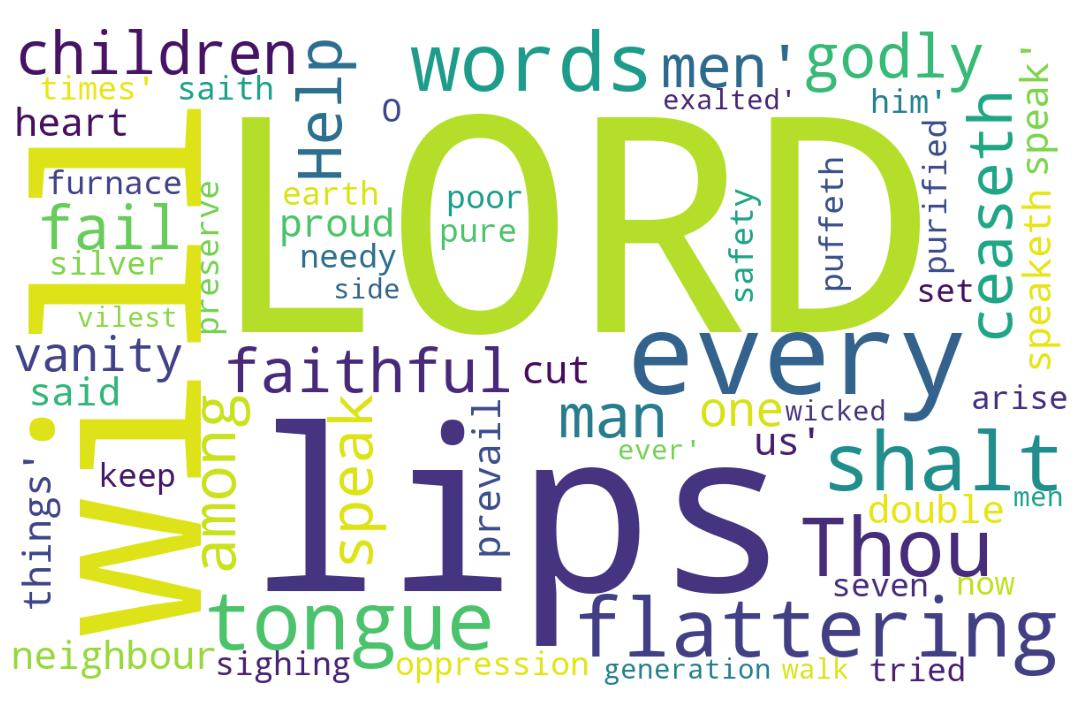
\includegraphics[width=\linewidth]{19OT-Psalms/Psalm12-WordCloud.jpg}
  \caption{Psalm 12 Word Cloud}
  \label{fig:Psalm 12 word Cloud}
\end{figure}


\marginpar{\scriptsize \centering \fcolorbox{bone}{lime}{\textbf{WORDS FROM THE LORD}}\\ (Psalm 12:1--8)     \begin{compactenum}[I.]
    \item \textbf{Provoked Words} \index[scripture]{Psalms!Psa 012:05}\index[scripture]{Psalms!Psa 012:01}(Psa 12:1, 5) (for the ...)
    \item \textbf{Proving Words} \index[scripture]{Psalms!Psa 012:05}(Psa 12:5) (now will I arise)
    \item \textbf{Protecting Words} \index[scripture]{Psalms!Psa 012:05}(Psa 12:5) (safety)
    \item \textbf{Prevailing Words} \index[scripture]{Psalms!Psa 012:05}(Psa 12:5) (Thou shall keep them)
    \item \textbf{Precious Words} \index[scripture]{Psalms!Psa 012:06}(Psa 12:6) (silver)
    \item \textbf{Preserved Words} \index[scripture]{Psalms!Psa 012:07}(Psa 12:7) (From this generation)
    \item \textbf{Permanent Words} \index[scripture]{Psalms!Psa 012:07}(Psa 12:7)
\end{compactenum}}

\textcolor[cmyk]{0.99998,1,0,0}{To the chief Musician upon Sheminith, A Psalm of David.}\\
\\
\footnote{\textcolor[cmyk]{0.99998,1,0,0}{\hyperlink{TOC}{Return to end of Table of Contents.}}}\footnote{\href{https://www.audioverse.org/english/audiobibles/books/ENGKJV/O/Ps/1}{\textcolor[cmyk]{0.99998,1,0,0}{Psalms Audio}}}\textcolor[cmyk]{0.99998,1,0,0}{Help, LORD; \fcolorbox{bone}{lime}{for the} godly man ceaseth; for the faithful fail from among the children of men.}
[2] \textcolor[cmyk]{0.99998,1,0,0}{They speak vanity every one with his neighbour: \emph{with} flattering lips \emph{and} with a double heart do they speak.}
[3] \textcolor[cmyk]{0.99998,1,0,0}{The LORD shall cut off all flattering lips, \emph{and} the tongue that speaketh proud things:}
[4] \textcolor[cmyk]{0.99998,1,0,0}{Who have said, With our tongue will we prevail; our lips \emph{are} our own: who \emph{is} lord over us?}
[5] \textcolor[cmyk]{0.99998,1,0,0}{\fcolorbox{bone}{lime}{For the} oppression of the poor, for the sighing of the needy, \fcolorbox{bone}{lime}{now will I arise}, saith the LORD; I will set \emph{him} in \fcolorbox{bone}{lime}{safety} \emph{from} \emph{him} \emph{that} puffeth at him.}\footnote{\textbf{Psalm 10:5} - His ways are always grievous; thy judgments are far above out of his sight: as for all his enemies, he puffeth at them.}\footnote{\textbf{1 Corinthians 8:1} - Now as touching things offered unto idols, we know that we all have knowledge. Knowledge puffeth up, but charity edifieth.}\footnote{\textbf{Job 3:24} - 
For my sighing cometh before I eat, and my roarings are poured out like the waters.}\footnote{\textbf{Psalm 31:10} - For my life is spent with grief, and my years with sighing: my strength faileth because of mine iniquity, and my bones are consumed.}\footnote{\textbf{Psalm 79:11} - Let the sighing of the prisoner come before thee; according to the greatness of thy power preserve thou those that are appointed to die;}\footnote{\textbf{Isaiah 35:1} - 
And the ransomed of the Lord shall return, and come to Zion with songs and everlasting joy upon their heads: they shall obtain joy and gladness, and sorrow and sighing shall flee away.}\footnote{\textbf{Jeremiah 45:3} - 
Thou didst say, Woe is me now! for the Lord hath added grief to my sorrow; I fainted in my sighing, and I find no rest.}
[6] \textcolor[cmyk]{0.99998,1,0,0}{The words of the LORD \emph{are} pure words: \emph{as} \fcolorbox{bone}{lime}{silver} tried in a furnace of earth, purified seven times.}
[7] \textcolor[cmyk]{0.99998,1,0,0}{Thou shalt keep them, O LORD, thou shalt \fcolorbox{bone}{lime}{preserve} them \fcolorbox{bone}{lime}{from this generation} for ever.}
[8] \textcolor[cmyk]{0.99998,1,0,0}{The wicked walk on every side, when the vilest men are exalted.}